\begin{frame}
  \centering
  \textbf{\Large{MRChem Software Suite}}
\end{frame}

\begin{frame}
\frametitle{MRChem software suite}
\scriptsize

\begin{columns}
\begin{column}[b]{0.4\linewidth}
\centering

\includegraphics[scale=0.12]{figures/mrchem.png}
\begin{itemize}
    \item Chemistry application
    \item High level C++
    \item MPI parallelized
\end{itemize}

\vspace{10mm}


\includegraphics[scale=0.1]{figures/mrcpp.png}
\begin{itemize}
    \item Multiwavelet library
    \item High performance C++
    \item OpenMP parallelized
\end{itemize}
\end{column}

\begin{column}[b]{0.40\linewidth}
\centering
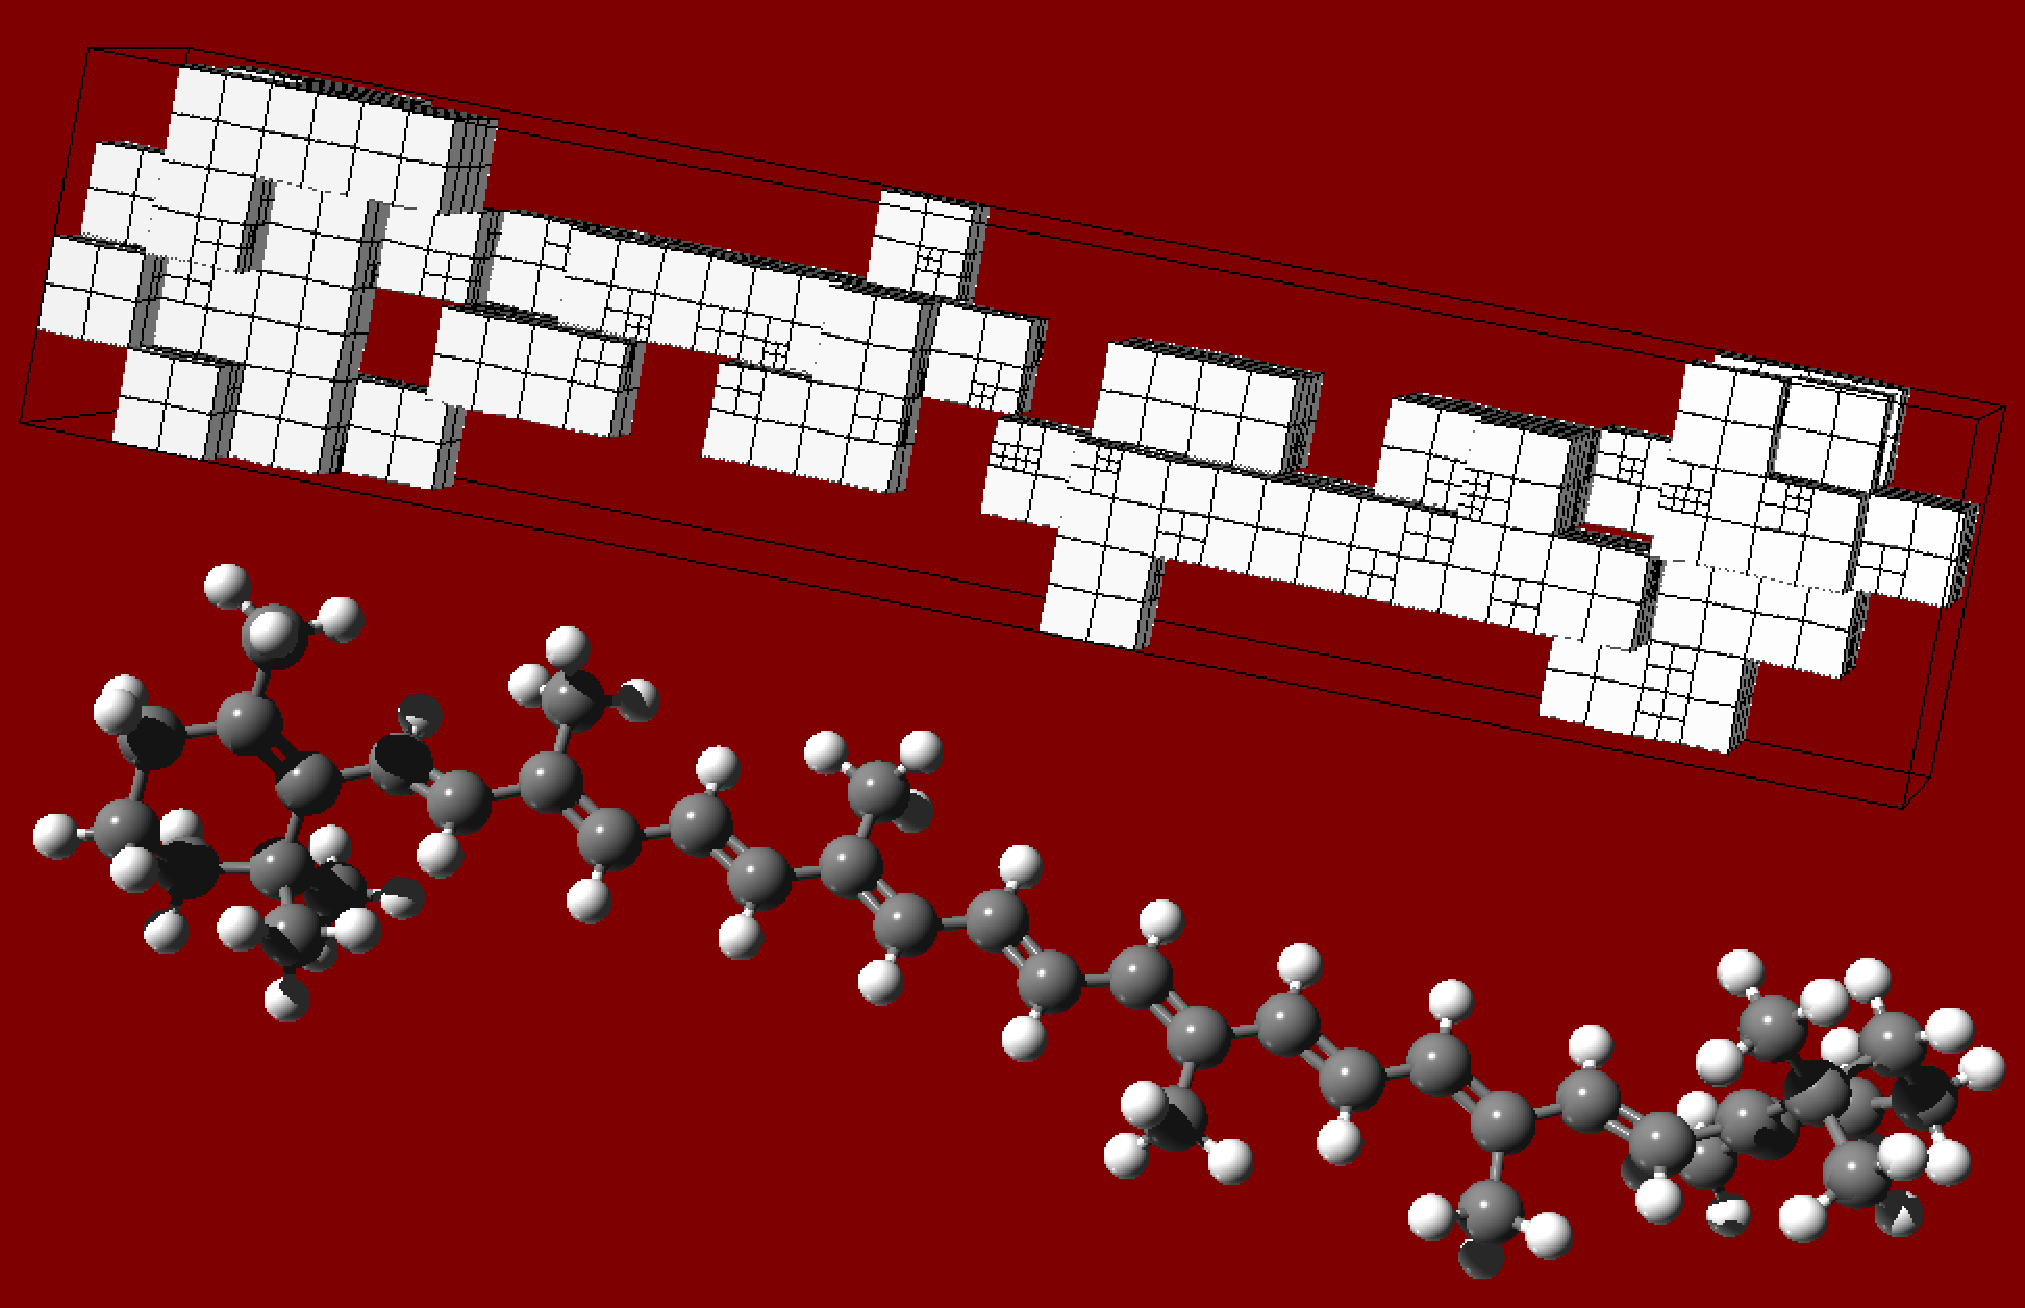
\includegraphics[scale=0.12]{figures/carotene_grid.pdf}\\

\vspace{12mm}


\includegraphics[scale=0.1]{figures/vampyr.png}
\begin{itemize}
    \item Interface to MRCPP
    \item High level Python
    \item Fast prototyping in Jupyter
\end{itemize}
\end{column}
\end{columns}

\end{frame}

%%%%%%%%%%%%%%%%%%%%%%%%%%%%%%%%%%%%%%%%%%%%%%%%%%%%%%%%%%%%%%%%%%%%%%%%%%%%%%%%

\begin{frame}
\frametitle{MRChem properties}
\small
\centering
\textbf{Methyloxirane molecule}
\hspace{30mm}
\textbf{Adaptive grid}
\begin{minipage}{0.5\textwidth}
\centering
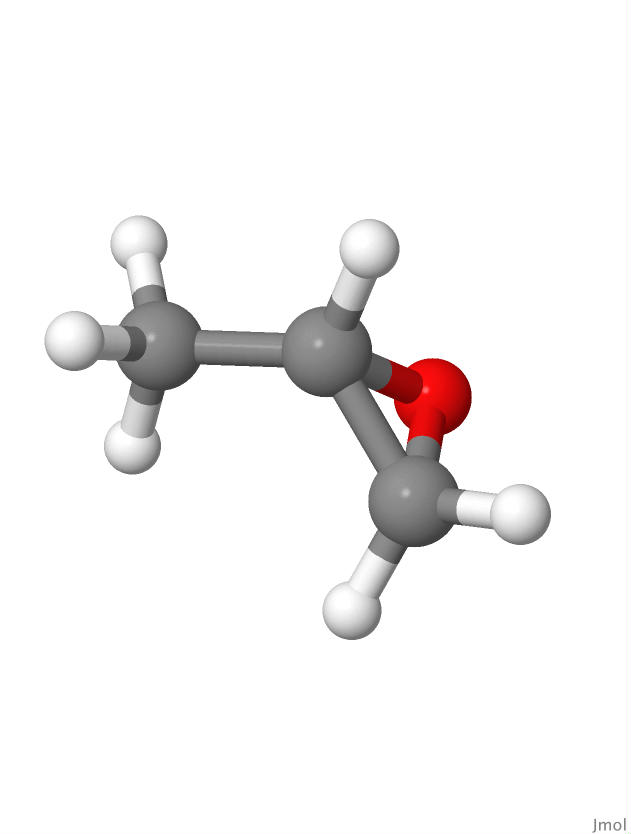
\includegraphics[scale=0.15, viewport = 0 180 550 650, clip]{figures/methyloxirane_white.jpg}
\end{minipage}%
\begin{minipage}{0.5\textwidth}
\centering
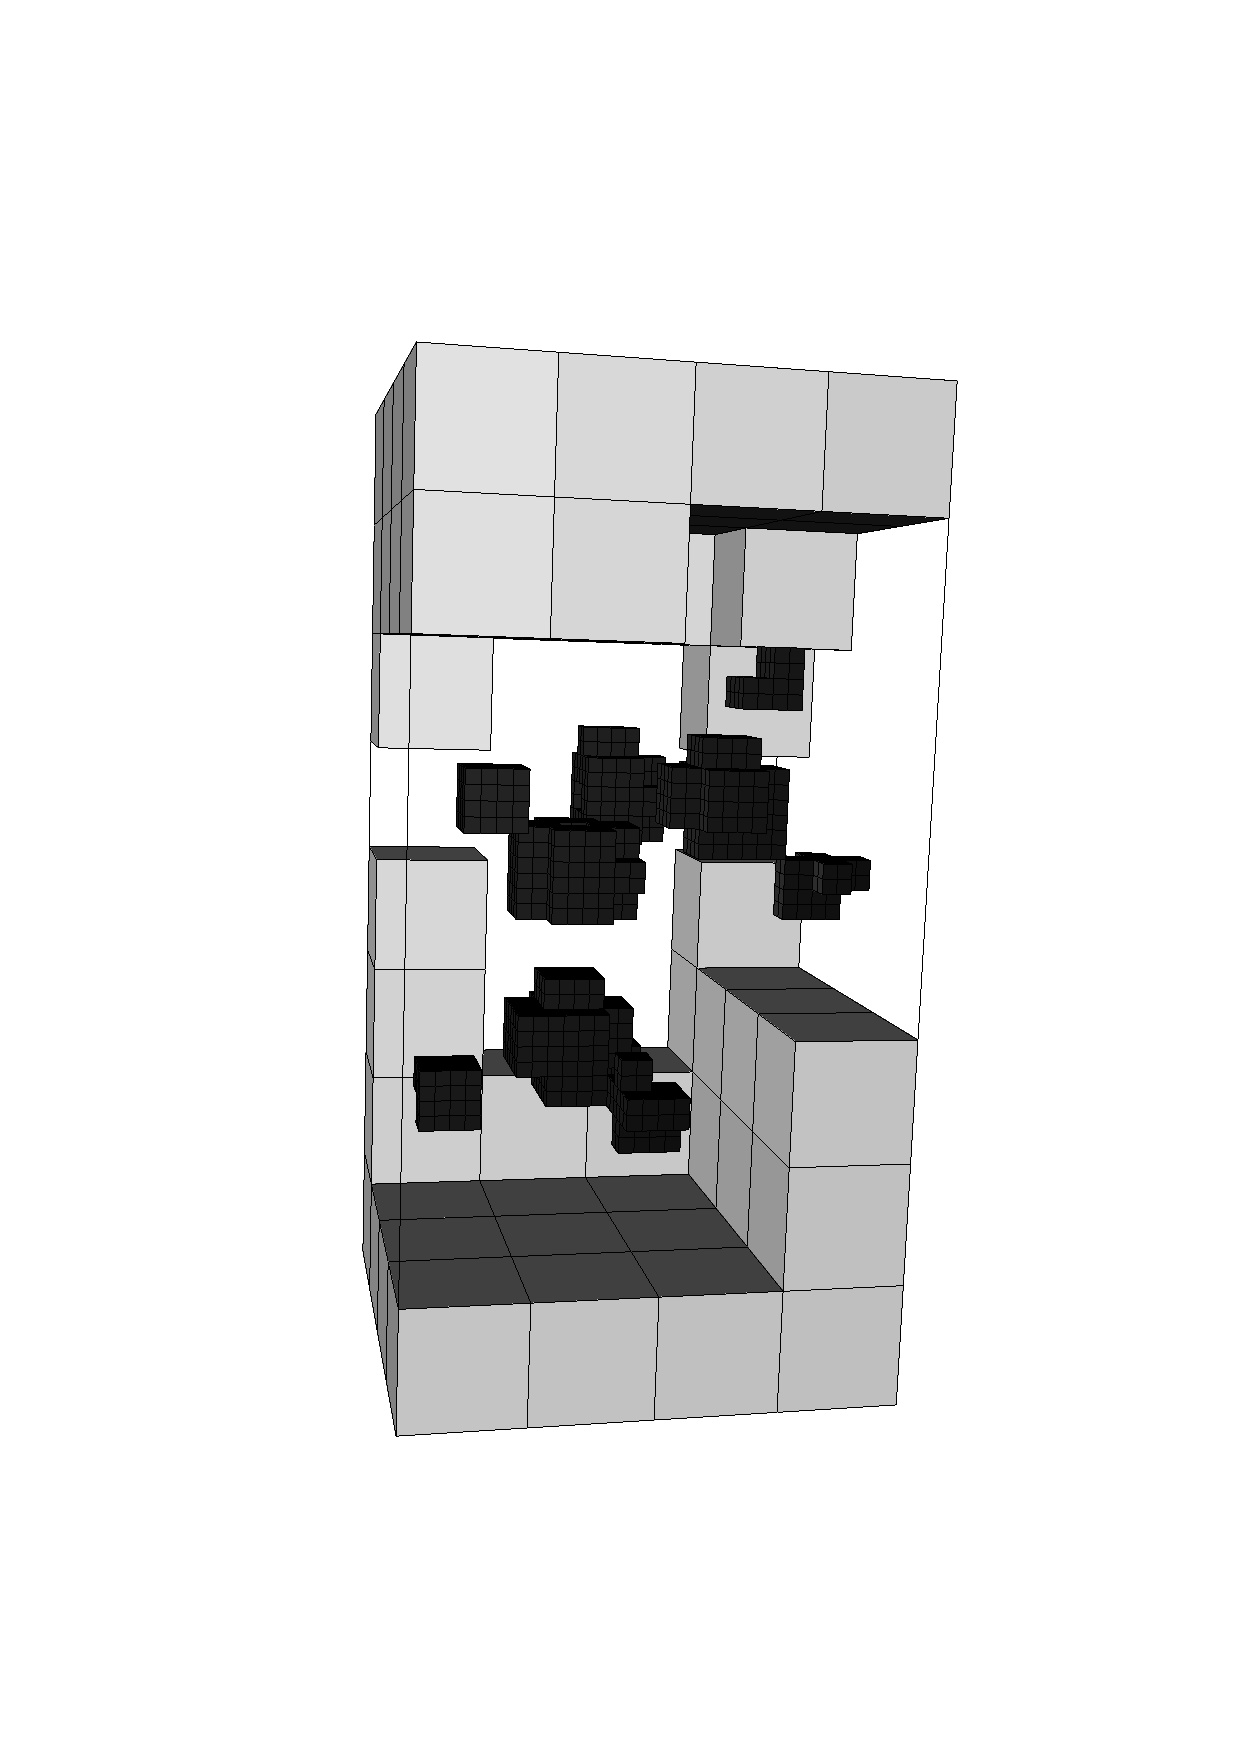
\includegraphics[angle=-90, scale=0.25, viewport = 170 150 470 700, clip]{figures/methyloxirane_grid.pdf}
\end{minipage}
\begin{table}
    \centering
    \textbf{Convergence of methyloxirane properties (a.u.) with PBE}
    \begin{tabular}{ccccc}
    \hline               
    \hline               
                   &                        &                 &                          &                  \\
\textbf{Precision} & \textbf{Energy}        & \textbf{Dipole} & \textbf{Magnetizability} & \textbf{NMR (O)} \\
    \hspace{10mm}\ & \hspace{20mm}\         & \hspace{15mm}\  & \hspace{15mm}\           & \hspace{15mm}\   \\
      MW4          & -192.9\red{70 600 312} & 0.72\red{0 854} & -9.23\red{7 441}         & 29\red{0.400}    \\
      MW5          & -192.963 \red{040 674} & 0.724 \red{527} & -9.241 \red{277}         & 292.\red{090}    \\
      MW6          & -192.962 95\red{8 847} & 0.725 0\red{47} & -9.241 2\red{08}         & 292.2\red{70}    \\
      MW7          & -192.962 955 \red{162} & 0.724 96\red{5} & -9.241 18\red{9}         & 292.29\red{2}    \\
      MW8          & -192.962 955 5\red{79} & 0.724 967       & -9.241 182               & 292.288          \\
                   &                        &                 &                          &                  \\
    \hline
    \hline
    \end{tabular}
\end{table}
\tiny
MWx: Multiwavelets with precision $\epsilon=10^{-x}$
\end{frame}


\begin{frame}
\frametitle{MRChem parallelization}

\centering
\textbf{Well suited for modern distributed architectures}

\begin{columns}
\begin{column}[b]{0.5\linewidth}

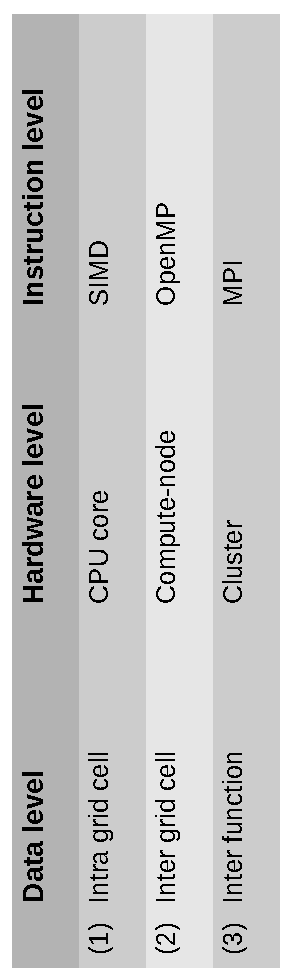
\includegraphics[scale=0.4, angle=-90]{figures/parallelization.pdf}

\vspace{0mm}

\end{column}

\begin{column}[b]{0.35\linewidth}

\begin{itemize}
    \item Molecule: $\sim 10^3$ orbitals
    \item Orbital: $\sim 10^3$ grid cells
    \item Grid cell: $\sim 10^3$ grid points
\end{itemize}

\vspace{2mm}

\end{column}
\end{columns}

\vspace{8mm}

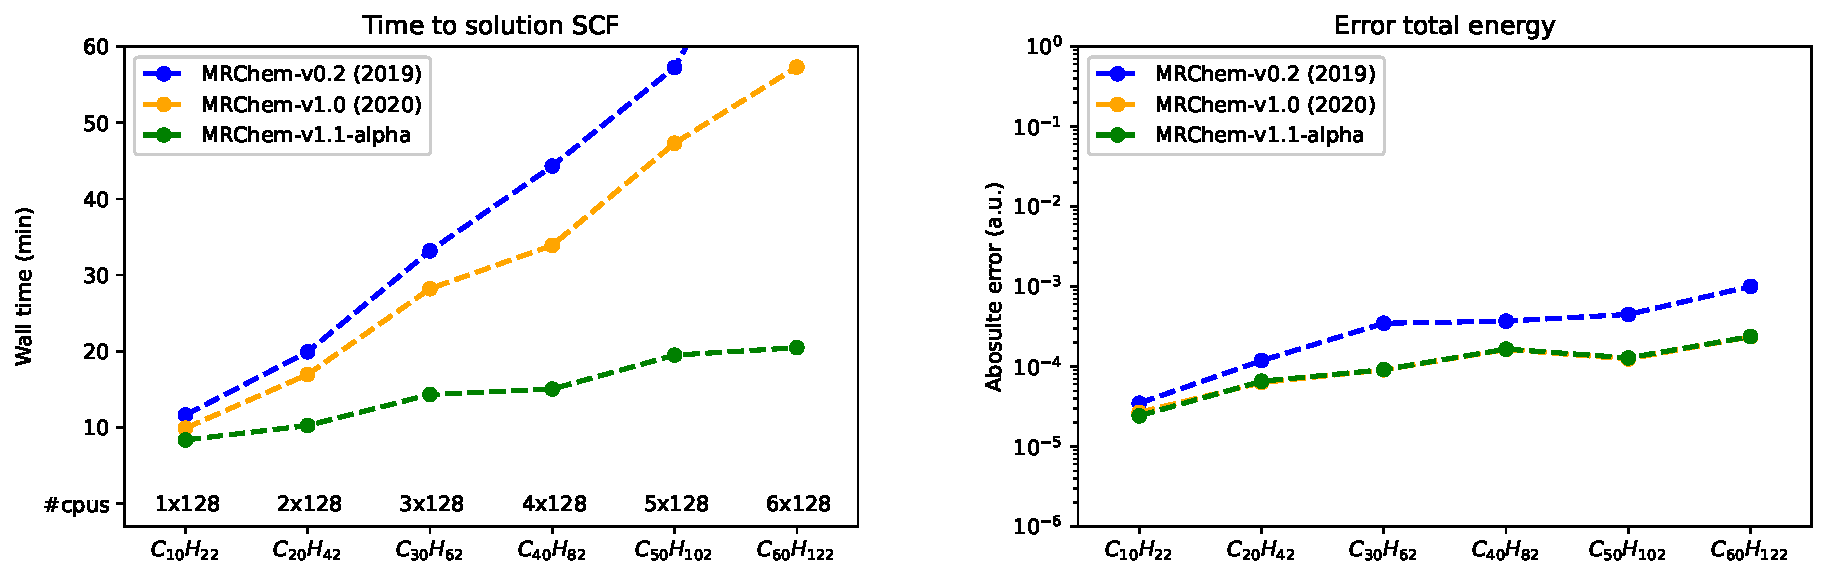
\includegraphics[scale=0.38]{figures/weak_scaling.pdf}

\end{frame}

%%%%%%%%%%%%%%%%%%%%%%%%%%%%%%%%%%%%%%%%%%%%%%%%%%%%%%%%%%%%%%%%%%%%%%%%%%%%%%%%

\begin{frame}
\frametitle{MRChem performance}

\begin{columns}
\begin{column}[b]{0.60\linewidth}
\centering
\textbf{Largest test case so far}
\begin{itemize}
    \item Gramicidin (C$_{198}$H$_{276}$N$_{40}$O$_{34}$, $\sim 2000$ electrons)
    \item Running on 84 Betzy nodes (10752 cores)
    \begin{itemize}
        %\small
        \item Hartree-Fock/MW4: $\sim 1$ min/cycle
        \item Hartree-Fock/MW5: $\sim 3$ min/cycle
        \item Hartree-Fock/MW6: $\sim 9$ min/cycle
    \end{itemize}
\end{itemize}

\vspace{5mm}

\end{column}

\begin{column}[b]{0.4\linewidth}

\vspace{-25mm}

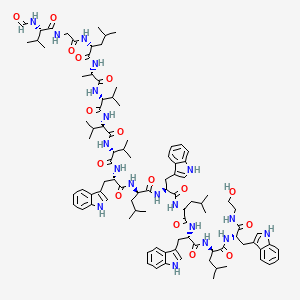
\includegraphics[scale=0.5]{figures/gramicidin.png}
\end{column}
\end{columns}

\centering
\textbf{Precision vs time to solution for SiH$_3$Cl}
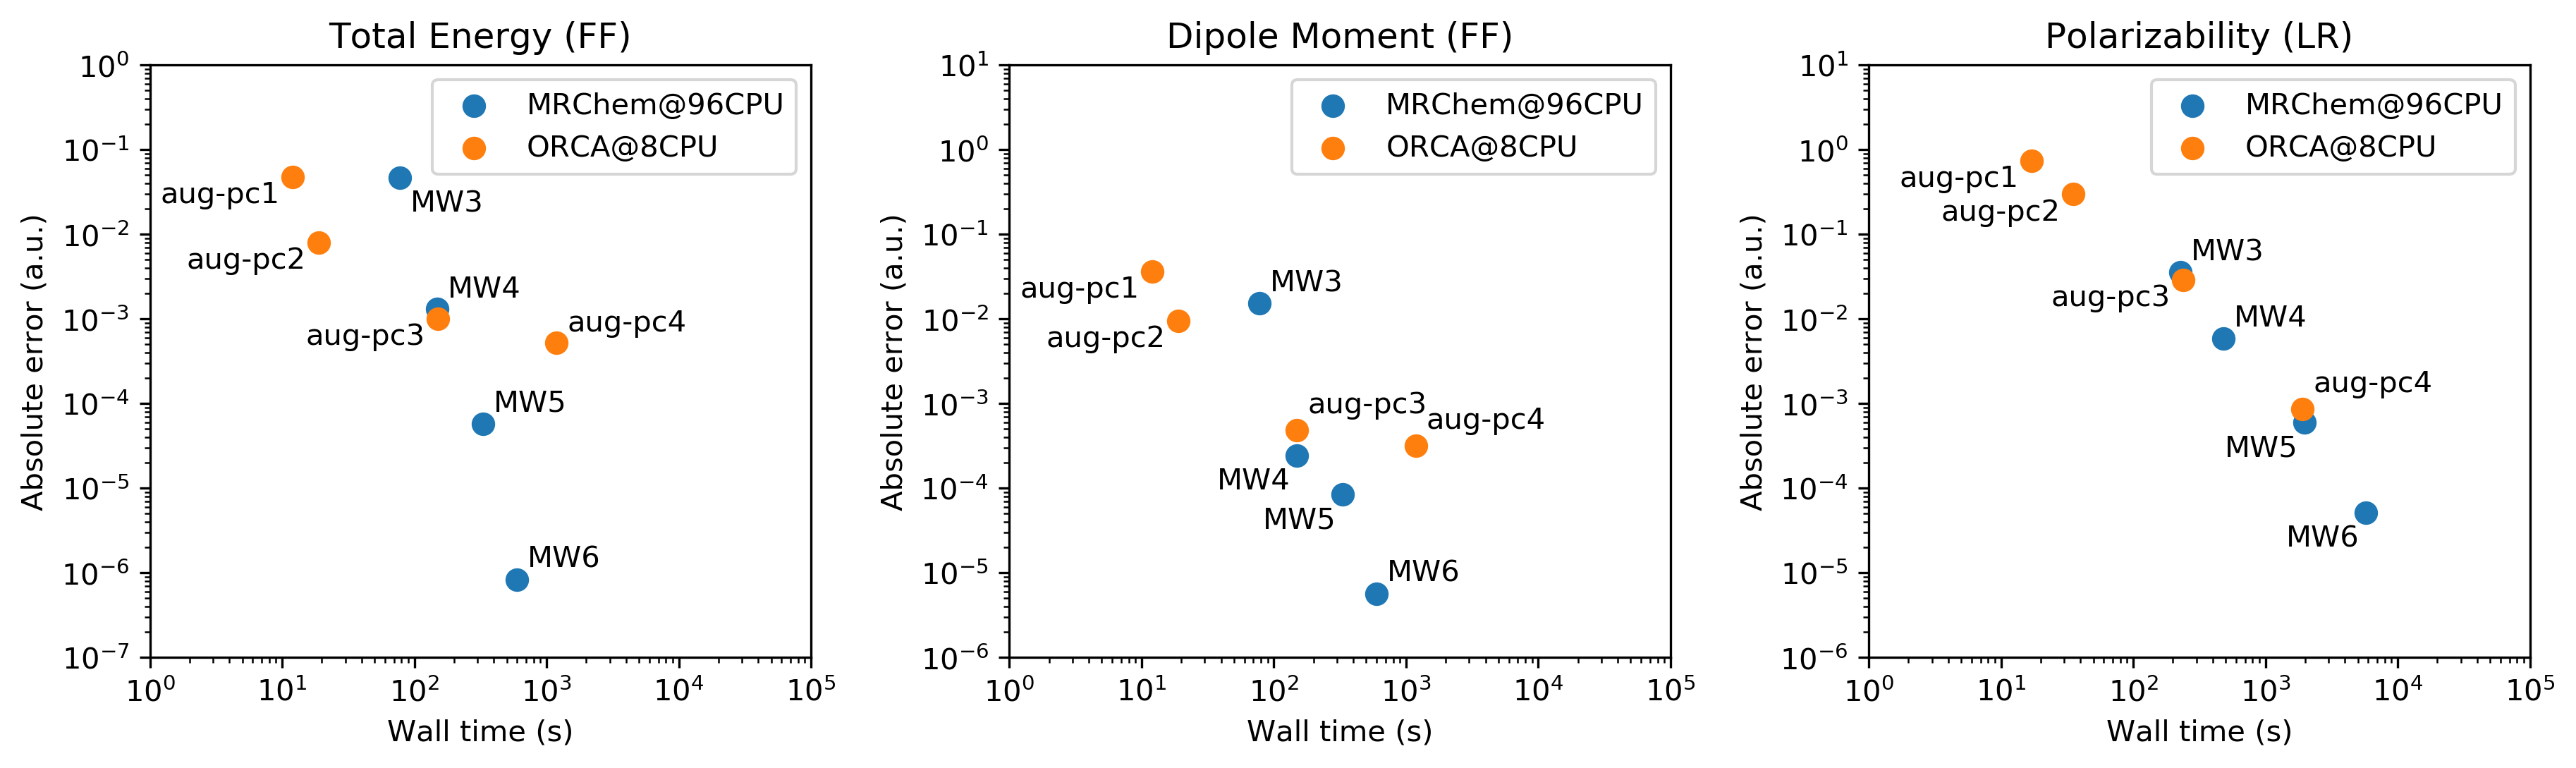
\includegraphics[scale=0.38]{figures/sih3cl.png}

\end{frame}

%%%%%%%%%%%%%%%%%%%%%%%%%%%%%%%%%%%%%%%%%%%%%%%%%%%%%%%%%%%%%%%%%%%%%%%%%%%%%%%%
